\documentclass{article}
\usepackage{neurips_2026}
\usepackage[utf8]{inputenc}
\usepackage[T1]{fontenc}
\usepackage{hyperref}
\usepackage{url}
\usepackage{booktabs}
\usepackage{amsfonts,amsmath,amssymb,amsthm}
\usepackage{nicefrac}
\usepackage{microtype}
\usepackage{xcolor}
\usepackage{graphicx}

\newcommand{\E}{\mathbb{E}}
\newcommand{\Var}{\mathrm{Var}}
\newcommand{\Cov}{\mathrm{Cov}}
\newtheorem{proposition}{Proposition}
\newtheorem{corollary}{Corollary}

\title{How Much Shorter Can Prediction-Powered Confidence Intervals Get? Headroom for the Mean When Labels, Unlabeled Data and Predictor Are Fixed}

\author{Anonymous Author(s)}

\begin{document}
\maketitle

\begin{abstract}
Prediction-powered inference (PPI) and its power-tuned variant PPI++ build valid confidence intervals from a small labeled sample, a large unlabeled sample and a fixed pretrained predictor. We ask how much shorter such intervals can be made when none of these three inputs may change. For the population mean we show that, among estimators that debias the predictor with any function of its output, PPI++ is optimal if and only if $\E[Y\mid f]$ is affine in the prediction $f$; PPI++ captures exactly a fraction $\rho^2=\mathrm{Corr}(\E[Y|f],f)^2$ of the variance reduction that $f$ can provide, and the remaining headroom has a closed form that can be estimated from data. We test nonlinear control variates (a natural-spline basis and cross-fitted isotonic regression) against classical, PPI, PPI++ and post-stratified intervals on nine real datasets (2000 resamples per setting) and eleven synthetic scenarios with known truth. The answer is conditional. On the real datasets the nonlinear controls shorten intervals by 0.6--1.2\% at $n=200$ and at most 0.6\% for $n\ge500$ relative to a PPI++ without the $[0,1]$ clipping of the tuning parameter, in line with a theoretical headroom below 2\%; larger differences to the reference \texttt{ppi\_py} implementation (up to 7\% on gene expression) are due to that clipping. On synthetic miscalibrated or non-monotone predictors, and on real outcomes whose predictor scores are put on a different monotone scale, widths shrink by 7--27\% (up to 35\% on re-scaled real scores) as predicted. At small $n$ the richer controls undercover with plain Wald intervals, which a degrees-of-freedom correction largely repairs, and under distribution shift a tuned $\lambda<1$ loses coverage that $\lambda=1$ keeps.
\end{abstract}

\section{Introduction}
Many scientific analyses have three ingredients: a small sample with gold-standard labels, a large sample with features only, and a pretrained predictor that cannot be modified. Prediction-powered inference \citep{angelopoulos2023ppi} and PPI++ \citep{angelopoulos2023ppipp} turn these into confidence intervals whose coverage does not depend on the predictor being accurate, and whose width shrinks when it is. Follow-up work changes the inputs: it trains the predictor on the labeled data with cross-fitting \citep{zrnic2023cross}, chooses which points to label \citep{zrnic2024active}, or exploits strata \citep{fisch2024stratified}.

We study a different question, with the inputs frozen: \emph{given the labeled set, the unlabeled set and the predictor, how much shorter can a valid interval for the mean be than the intervals available today, and when?} The question matters because labels are the bottleneck and any width reduction at no extra cost is worth having; it is also easy to answer wrongly, since a narrower interval that undercovers is not a gain.

\paragraph{Contributions.}
(i) A short exact analysis (Section~\ref{sec:theory}) of the class of estimators $\hat\theta_h=\bar Y_L-(\bar h_L-\bar h_U)$ with arbitrary $h(f)$: the optimal $h$ is a shrunken regression function $\tfrac{N}{n+N}\E[Y|f]$; PPI++ is optimal iff $\E[Y|f]$ is affine in $f$; PPI++ realises a fraction $\rho^2$ of the possible variance reduction over the classical interval; and the reference implementation's clipping of $\lambda$ costs width when the predictor's scale is small. (ii) Two simple estimators with nonlinear controls and a degrees-of-freedom-corrected variant (Section~\ref{sec:methods}); they are mild extensions of PPI++, not a new inference principle. (iii) An empirical evaluation with repeated sampling, uncertainty on both coverage and width, and a theory-versus-experiment check (Section~\ref{sec:exp}), including negative and failure cases: no gain on real predictors that are already near-affinely calibrated, undercoverage at small $n$, and fragility of tuned estimators under shift.

\section{Related work}
PPI \citep{angelopoulos2023ppi} debiases predictions on unlabeled data with a rectifier estimated on labeled data; PPI++ \citep{angelopoulos2023ppipp} adds a data-driven tuning parameter $\lambda$ that interpolates between PPI and the classical estimator and covers means, quantiles and regression. Cross-prediction \citep{zrnic2023cross} handles predictors trained on the same labeled data; active inference \citep{zrnic2024active} and stratified PPI \citep{fisch2024stratified} change which points are labeled. Our setting differs in that nothing about data collection or the predictor changes. Our nonlinear controls use the cross-fitting idea from double/debiased machine learning \citep{chernozhukov2016dml} for a one-dimensional nuisance $\E[Y|f]$. The control-variate structure used here is the one underlying PPI++ with a vector tuning parameter; what we add is the quantification of what is left after the optimal scalar tuning for the mean. We did not read the full texts of the cited works beyond their abstracts and, for \texttt{ppi\_py}, its source code; statements about them are limited to what the abstracts and the code state.

\section{Setting and headroom analysis}\label{sec:theory}
\paragraph{Setting.} Labeled pairs $(f_i,Y_i)_{i\le n}$ and unlabeled predictions $(f_j)_{j\le N}$ are i.i.d.\ from one distribution; $f=f(\text{features})$ is the output of the fixed predictor. The target is $\theta=\E Y$ (chosen because it has a closed-form analysis, is the primary target of all cited methods, and is the simplest quantity on which to test whether any room is left). Write $g(f)=\E[Y|f]$, $v(f)=\Var(Y|f)$. For any $h$ with $\E h(f)^2<\infty$ define
\begin{equation}\label{eq:est}
\hat\theta_h=\frac1n\sum_{i\le n}\big(Y_i-h(f_i)\big)+\frac1N\sum_{j\le N}h(f_j).
\end{equation}
Classical: $h\equiv0$; PPI: $h=f$; PPI++: $h=\lambda f$ with tuned $\lambda$. (Using the labeled $f_i$ also in the second mean only re-parametrises $\lambda$ and gives nothing new.)

\begin{proposition}\label{prop:main}
$\hat\theta_h$ is unbiased with asymptotic (and, for fixed $h$, exact) variance $V(h)=\Var(Y-h)/n+\Var(h)/N$. With $c=N/(n+N)$,
\[
V(h)=V_\star+\Big(\frac1n+\frac1N\Big)\Var\big(h(f)-c\,g(f)\big),\qquad V_\star=\frac{\E v(f)}{n}+\frac{\Var g(f)}{n+N}.
\]
Hence $h_\star=c\,g$ minimises $V$ over all $h$, with minimum $V_\star$.
\end{proposition}

\begin{corollary}[Headroom beyond PPI++]\label{cor:lin}
Let $\rho=\mathrm{Corr}(g(f),f)$. The best $h=\lambda f$ (PPI++ with unclipped $\lambda^\star=\Cov(g,f)/((1+n/N)\Var f)$) has $V_{\rm lin}=V_\star+\frac{N}{n(n+N)}\Var(g)(1-\rho^2)$. The classical variance $V_0=\Var(Y)/n$ satisfies $V_0-V_\star=\frac{N}{n(n+N)}\Var g$, so PPI++ achieves a fraction $\rho^2$ of the variance reduction available from $f$. Equivalently $V_{\rm lin}/V_\star=1+\Gamma$ with $\Gamma=\frac{N\,\Var g\,(1-\rho^2)}{(n+N)\E v+n\Var g}$, and the asymptotic width ratio of the optimal nonlinear control to PPI++ is $(1+\Gamma)^{-1/2}$. In particular no gain is possible iff $g$ is almost surely affine in $f$ (e.g.\ any predictor taking two values), and the maximal gain is attained when $\rho=0$.
\end{corollary}

\begin{corollary}[Clipping]\label{cor:clip}
$V(\lambda f)=V(\lambda^\star f)+(\tfrac1n+\tfrac1N)\Var(f)(\lambda-\lambda^\star)^2$. The reference implementation \texttt{ppi\_py} (v0.2.3) clips the tuned $\lambda$ to $[0,1]$ (we read its source); when $\lambda^\star>1$, e.g.\ for predictors on a smaller scale than $Y$, clipping costs the excess above.
\end{corollary}

Proofs are in Appendix~\ref{app:proofs}. The minimiser $V_\star$ coincides with the asymptotic variance of the unique influence function when labels are missing completely at random with known probability and $f$ is always observed; we use $V_\star$ as the benchmark for ``how short can it get'' and argue (without a full proof, Appendix~\ref{app:proofs}) that it cannot be beaten by regular estimators of this information structure. The corollaries give three sources of possible shortening relative to the \texttt{ppi\_py} PPI++: (a) removing the clip, (b) nonlinear $h$, and (c) nothing beyond $V_\star$. They also give a data-based diagnostic: estimate $\E v$, $\Var g$, $\rho$ from the labeled data and compute $\Gamma$ before changing the estimator. \emph{Finite samples:} the controls must be estimated; with $p$ estimated coefficients the plug-in Wald interval is expected to be too short by a relative amount of order $p/n$, which is why we also report $t$-corrected versions.

\section{Estimators compared}\label{sec:methods}
All intervals are $\hat\theta\pm z_{.975}\widehat{\mathrm{se}}$ unless stated.
\textbf{Classical:} $\bar Y_L$ with $s/\sqrt n$. \textbf{PPI} ($\lambda=1$) and \textbf{PPI++} via \texttt{ppi\_py} 0.2.3 (\citealp{ppipy}; PPI++ uses its default tuned and clipped $\lambda$; our own PPI $\lambda=1$ implementation agrees with the package, see \texttt{code/test\_methods.py}). \textbf{PPI++ unclipped:} our implementation of the plug-in optimal $\lambda$ without clipping.
\textbf{Post-stratified PPI (K=5):} $\lambda=1$ within five equal-mass strata of the pooled predictions, an adaptation of the stratification idea of \citet{fisch2024stratified} to simple random labeling (not their allocation scheme); the standard error accounts for the random stratum shares.
\textbf{NC-spline PPI++:} control $H(f)\in\mathbb R^{k-1}$ from a natural cubic spline with $k$ knots at pooled-prediction quantiles (dummy coding if $f$ has $\le k+2$ distinct values); vector $\lambda=(\hat\Sigma_L+\tfrac nN\hat\Sigma_U)^{-1}\hat c$, $\hat\theta=\bar Y-\lambda^\top(\bar H_L-\bar H_U)$, $\widehat{\mathrm{se}}^2=\widehat\Var(Y-\lambda^\top H)/n+\lambda^\top\hat\Sigma_U\lambda/N$. The span contains $f$, so it is asymptotically never worse than PPI++. $k=4$ was the default fixed before seeing real-data results; $k=3,6$ are sensitivity checks.
\textbf{CF-isotonic:} $h=\hat g^{(-k)}(f)$ from 5-fold cross-fitted isotonic regression (monotone direction chosen automatically), scalar $\lambda$ as above (asymptotically $h_\star$ if $g$ is monotone).
\textbf{$t$-corrected variants} (classical, PPI++ unclipped, NC-spline $k{=}4$): residual variance divided by $n-p-1$ instead of $n-1$ and Student-$t_{n-p-1}$ critical value ($t_{n-1}$ for classical).

\section{Experiments}\label{sec:exp}
\paragraph{Protocol.} \emph{Real data:} the nine \texttt{ppi-python} example collections (v0.2.3; \citealt{ppipy}) with their stored $(Y,\hat Y)$ pairs: galaxy spiral-arm presence, forest loss, AlphaFold disorder, gene expression, census income / private insurance / education (each from a pool of $>3\times10^5$ records), plankton and ballots (the stored labeled parts). Each pool is treated as the population; the truth is the pool mean of $Y$; in each of $R=2000$ replications $n$ labeled points and $N=10^4$ unlabeled points are drawn i.i.d.\ \emph{with replacement} from the pool ($n\in\{50,100,200,500,1000,2000\}$; up to 500 for the small pools forest and ballots). This makes the i.i.d.\ assumption hold exactly for the empirical distribution; it also means for small pools that the unlabeled sample contains repeats. \emph{Synthetic:} $f\sim N(0,1)$, $Y=g(f)+\varepsilon$ with known truth: Hermite scenarios $g=\cos\phi\,f+\sin\phi\,(f^2-1)/\sqrt2$ ($\phi\in\{0^\circ,30^\circ,60^\circ,90^\circ\}$, $\rho^2=\cos^2\phi$, $\varepsilon\sim N(0,1)$), lognormal $g\propto e^{\beta f}$ ($\beta\in\{1,1.5\}$), logistic Bernoulli outcomes $g=\mathrm{expit}(-1+bf)$ ($b\in\{1,3\}$), a binary predictor, and two scenarios with $f$ shrunk by 0.25 ($R=2000$ each, $n\in\{50,\dots,1000\}$, $N=10^4$; $N\in\{200,10^3,10^5\}$ at $n=200$ are in the released CSV). \emph{Metrics:} empirical coverage with Wilson 95\% intervals (half-width $\approx1$ point at $R=2000$); mean width and the \emph{paired} per-replication width ratio to PPI++ (\texttt{ppi\_py}) with its standard error; theory columns use Corollary~\ref{cor:lin} (synthetic: exact moments by quadrature; real: $\E v$ from 10-fold cross-fitted gradient boosting on the pool, so the headroom is, if anything, understated). No multiplicity correction is applied: results are descriptive, and claims rest on patterns across many settings rather than on single tests.

\begin{figure}[t]
\centering
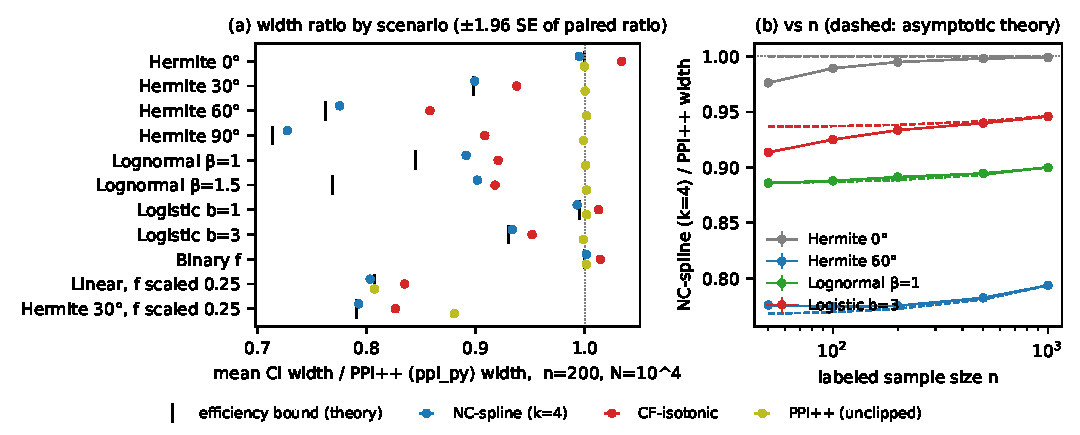
\includegraphics[width=\linewidth]{figs/fig_synth_width.pdf}
\caption{Synthetic scenarios with known truth ($N=10^4$, $R=2000$). (a) Mean width relative to PPI++ (\texttt{ppi\_py}) at $n=200$; bars $\pm1.96$ paired SE; black ticks: asymptotic efficiency bound $\sqrt{V_\star/V_{\rm PPI++}}$. (b) Dependence on $n$; dashed: asymptotic prediction for the NC-spline ($k=4$) control. Generated by \texttt{code/make\_figs.py}.}\label{fig:synth}
\end{figure}

\paragraph{Synthetic results: gains exist, as predicted, when $g$ is not affine.}
Figure~\ref{fig:synth} and Table~\ref{tab:synth} show the width of the NC-spline control relative to PPI++. With affine $g$ (Hermite $0^\circ$, binary predictor, weakly nonlinear logistic $b{=}1$) the ratio is $0.995$--$1.001$, matching the theoretical $1$. With nonlinear $g$ it is $0.899$ ($30^\circ$), $0.775$ ($60^\circ$) and $0.727$ ($90^\circ$, a purely quadratic signal on which PPI++ equals the classical interval), against bounds $0.898$, $0.762$, $0.714$; for lognormal and logistic $b{=}3$ it is $0.891$/$0.902$/$0.933$ against bounds $0.845$/$0.769$/$0.930$. For the heavy exponential $g$ ($\beta=1.5$) the 4-knot spline recovers less than half of the available reduction (0.902 vs.\ bound 0.769), while the cross-fitted isotonic control improves with $n$ (0.918 at $n=200$, 0.866 at $n=1000$). The dependence on $N$ also follows Corollary~\ref{cor:lin}: for Hermite $60^\circ$ at $n=200$ the NC-spline ratio is 0.897, 0.817, 0.775, 0.770 for $N=200,10^3,10^4,10^5$ (asymptotic prediction 0.899, 0.815, 0.773, 0.767). Panel (b) shows the asymptotic prediction tracking the empirical ratios. When $f$ is on a smaller scale than $Y$ (last two rows), most or all of the gain over \texttt{ppi\_py} comes from removing the $\lambda$ clip: unclipped PPI++ is already $0.807$ for the linear case. Coverage of the NC-spline at $n=200$ is within $[0.935,0.952]$ in all scenarios. The number of knots matters little (Table~\ref{tab:sens}): $k=6$ is 1--6 points narrower than $k=3$ for nonlinear $g$ and up to 1.4 points lower in coverage at $n=100$; $k=4$ is a compromise and was not tuned. Across the 11 scenarios $\times$ five $n$ (Table~\ref{tab:cover}) the worst coverage is $0.912$ for the NC-spline at $n=50$ (0.927 with the $t$ correction).

\begin{table}[t]
\centering\small
\caption{Synthetic scenarios, $n=200$, $N=10^4$, $R=2000$: mean CI width divided by that of PPI++ (\texttt{ppi\_py}); columns PPI, PPI++ unclip., NC-spline ($k{=}4$) and CF-iso are empirical; Bound is the asymptotic efficiency bound $\sqrt{V_\star/V_{\rm PPI++}}$; last two columns: empirical coverage (nominal 0.95).}\label{tab:synth}
\begin{tabular}{lrrrrrrr}
\toprule
Scenario & PPI & PPI++ unclip. & NC-spline & CF-iso & Bound & cov. PPI++ & cov. NC-spline \\
\midrule
Hermite 0$^\circ$ & 1.002 & 1.000 & 0.995 & 1.034 & 1.000 & 0.958 & 0.952 \\
Hermite 30$^\circ$ & 1.014 & 1.000 & 0.899 & 0.938 & 0.898 & 0.944 & 0.943 \\
Hermite 60$^\circ$ & 1.084 & 1.002 & 0.775 & 0.858 & 0.762 & 0.946 & 0.949 \\
Hermite 90$^\circ$ & 1.238 & 0.999 & 0.727 & 0.908 & 0.714 & 0.948 & 0.949 \\
Lognormal $\beta$=1 & 1.035 & 1.001 & 0.891 & 0.921 & 0.845 & 0.941 & 0.944 \\
Lognormal $\beta$=1.5 & 1.108 & 1.002 & 0.902 & 0.918 & 0.769 & 0.940 & 0.936 \\
Logistic b=1 & 2.213 & 1.002 & 0.993 & 1.013 & 0.995 & 0.948 & 0.946 \\
Logistic b=3 & 2.140 & 0.999 & 0.933 & 0.952 & 0.930 & 0.949 & 0.950 \\
Binary f & 1.137 & 1.001 & 1.001 & 1.014 & 1.000 & 0.942 & 0.942 \\
Linear, f scaled 0.25 & 1.003 & 0.807 & 0.803 & 0.835 & 0.807 & 0.936 & 0.935 \\
Hermite 30$^\circ$, f scaled 0.25 & 1.003 & 0.880 & 0.793 & 0.826 & 0.791 & 0.945 & 0.942 \\
\bottomrule
\end{tabular}
\end{table}

\begin{table}[t]
\centering\small
\caption{Sensitivity to the number of spline knots $k$: width ratio to PPI++ (\texttt{ppi\_py}) at $n=200$, coverage at $n=100$ ($N=10^4$, $R=2000$); Bound as in Table~\ref{tab:synth}. The last row averages the seven real datasets with continuous scores.}\label{tab:sens}
\resizebox{\linewidth}{!}{\begin{tabular}{lrrrrrrr}
\toprule
 & \multicolumn{3}{c}{width ratio, $n{=}200$} & \multicolumn{3}{c}{coverage, $n{=}100$} & \\
Setting & $k{=}3$ & $k{=}4$ & $k{=}6$ & $k{=}3$ & $k{=}4$ & $k{=}6$ & Bound \\
\midrule
Hermite 0$^\circ$ & 0.997 & 0.995 & 0.990 & 0.943 & 0.939 & 0.931 & 1.000 \\
Hermite 30$^\circ$ & 0.904 & 0.899 & 0.893 & 0.945 & 0.940 & 0.931 & 0.898 \\
Hermite 60$^\circ$ & 0.783 & 0.775 & 0.766 & 0.943 & 0.939 & 0.929 & 0.762 \\
Hermite 90$^\circ$ & 0.736 & 0.727 & 0.717 & 0.947 & 0.945 & 0.942 & 0.714 \\
Lognormal $\beta$=1 & 0.916 & 0.891 & 0.876 & 0.934 & 0.927 & 0.925 & 0.845 \\
Lognormal $\beta$=1.5 & 0.935 & 0.902 & 0.878 & 0.941 & 0.941 & 0.930 & 0.769 \\
Logistic b=3 & 0.977 & 0.933 & 0.920 & 0.931 & 0.936 & 0.932 & 0.930 \\
Binary f & 1.001 & 1.001 & 1.001 & 0.945 & 0.945 & 0.945 & 1.000 \\
\midrule
Real, 7 continuous-score datasets (mean) & 0.982 & 0.979 & 0.975 & 0.921 & 0.918 & 0.914 & -- \\
\bottomrule
\end{tabular}}
\end{table}

\paragraph{Real datasets: almost nothing left once $\lambda$ is unclipped.}
Table~\ref{tab:real} and Figure~\ref{fig:real} show the real-data widths. The theoretical bound $V_\star$ computed from the pools is within $2\%$ of the unclipped PPI++ width for every dataset at $n=200$ (largest headroom: forest $0.983$, gene expression $0.989$, AlphaFold $0.991$, others $\ge0.997$), because the stored predictors are nearly affinely calibrated on the pool ($\rho^2\ge0.99$ for 8 of 9 datasets, $0.908$ for forest; Table~\ref{tab:pool}). Empirically the NC-spline interval is $0.6$--$1.2\%$ shorter than unclipped PPI++ at $n=200$ on the seven datasets with continuous scores, and $0.2$--$0.6\%$ shorter at $n=500$ (ratios of mean widths), which is what the bound allows; part of the $n=200$ difference is small-sample optimism of the plug-in standard error (see below). CF-isotonic is $1.5$--$3.4\%$ \emph{wider} than PPI++ at $n=200$ on these datasets (gene expression: $2.5\%$ narrower) and converges to it only for $n\gtrsim1000$, i.e.\ the price of estimating $g$ nonparametrically exceeds the available gain. Post-stratified PPI is $0.4$--$1.6\%$ wider than PPI++ at $n=200$ on these datasets (gene expression: $4.9\%$ narrower), and its width grows relative to PPI++ with $n$ (e.g.\ $+6.3\%$ on gene expression at $n=2000$). Relative to the \texttt{ppi\_py} PPI++, however, two datasets show visible differences: gene expression (unclipped PPI++ $0.938$ of the width at $n=200$, $0.886$ at $n=50$, $0.971$ at $n=500$) and census income ($0.979$ at $n=200$), where $\lambda^\star>1$ and the clip binds; this is Corollary~\ref{cor:clip} at work, not nonlinearity (the nonlinear headroom beyond unclipped PPI++ is $\le1.2\%$ there). The classical interval is $1.2$--$4.6\times$ wider than PPI++ across datasets at $n=200$, so the benefit of PPI itself is large; the benefit of going further is not. On plankton and ballots the predictor is binary and all of PPI++ unclipped, NC-spline and (nearly) CF-isotonic coincide, as the theory requires.

\begin{table}[t]
\centering\small
\caption{Real datasets: mean CI width relative to PPI++ (\texttt{ppi\_py}) (ratio of paired widths averaged over $R=2000$ resamples, $N=10^4$). Bound: asymptotic efficiency bound at that $n$. Values below 1 are not gains if coverage is lost; see Table~\ref{tab:cover}.}\label{tab:real}
\resizebox{\linewidth}{!}{\begin{tabular}{llrrrrrrr}
\toprule
Dataset & $n$ & Classical & PPI & PPI++ unclip. & Post-strat & NC-spline & CF-iso & Bound \\
\midrule
Galaxies & 200 & 1.486 & 1.002 & 0.999 & 1.013 & 0.992 & 1.030 & 0.998 \\
Galaxies & 1000 & 1.414 & 1.008 & 1.000 & 1.008 & 0.999 & 1.007 & 0.998 \\
Forest & 200 & 1.187 & 1.006 & 0.999 & 1.015 & 0.992 & 1.015 & 0.983 \\
Forest & 500 & 1.177 & 1.006 & 0.999 & 1.006 & 0.996 & 1.002 & 0.984 \\
AlphaFold & 200 & 1.724 & 0.997 & 0.994 & 1.006 & 0.985 & 1.033 & 0.991 \\
AlphaFold & 1000 & 1.590 & 1.002 & 0.999 & 1.008 & 0.997 & 1.005 & 0.993 \\
Gene expr. & 200 & 3.145 & 1.000 & 0.938 & 0.951 & 0.931 & 0.975 & 0.930 \\
Gene expr. & 1000 & 2.516 & 1.000 & 0.994 & 1.021 & 0.992 & 0.997 & 0.989 \\
Census income & 200 & 1.258 & 1.002 & 0.979 & 1.004 & 0.967 & 1.030 & 0.979 \\
Census income & 1000 & 1.220 & 1.000 & 0.990 & 0.999 & 0.986 & 1.006 & 0.988 \\
Census health & 200 & 1.408 & 1.003 & 1.001 & 1.016 & 0.994 & 1.028 & 0.999 \\
Census health & 1000 & 1.355 & 1.006 & 1.000 & 1.006 & 0.999 & 1.008 & 1.000 \\
Census educ. & 200 & 1.286 & 1.004 & 0.999 & 1.015 & 0.993 & 1.034 & 0.999 \\
Census educ. & 1000 & 1.249 & 1.005 & 1.000 & 1.007 & 0.999 & 1.011 & 0.999 \\
Plankton & 200 & 1.830 & 1.032 & 0.983 & 0.998 & 0.983 & 1.004 & 1.000 \\
Plankton & 1000 & 1.659 & 1.075 & 0.997 & 1.009 & 0.997 & 1.001 & 1.000 \\
Ballots & 200 & 4.646 & 1.007 & 0.991 & 0.999 & 0.991 & 0.999 & 1.000 \\
Ballots & 500 & 3.524 & 1.029 & 0.998 & 1.014 & 0.998 & 1.000 & 1.000 \\
\bottomrule
\end{tabular}}
\end{table}

\begin{figure}[t]
\centering
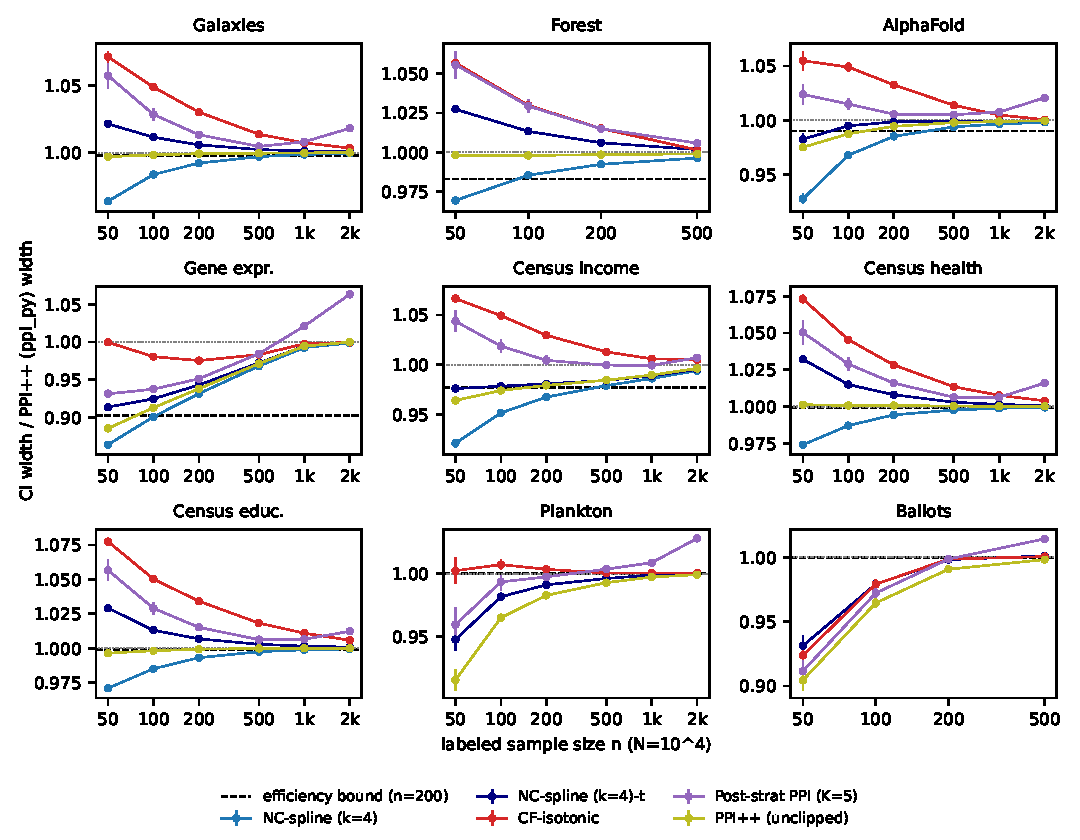
\includegraphics[width=\linewidth]{figs/fig_real_width.pdf}
\caption{Real datasets: mean width relative to PPI++ (\texttt{ppi\_py}) vs $n$ ($N=10^4$, $R=2000$; $\pm1.96$ paired SE). Dashed: asymptotic efficiency bound at $n=200$. Curves of the plain NC-spline below 1 at small $n$ are accompanied by undercoverage (Table~\ref{tab:cover}); the $t$-corrected variant (dark blue) is wider.}\label{fig:real}
\end{figure}

\paragraph{Validity: the apparent small-$n$ gains are largely not real.}
Table~\ref{tab:cover} and Figure~\ref{fig:cover} summarise coverage. For $n\ge500$ all intervals are close to nominal (mean 0.947--0.949 over settings), with isolated deviations on the heavy-tailed census income target (0.93--0.94 at $n=500$--$1000$). For $n\le100$ the plug-in Wald intervals undercover on real data: classical $0.934$, PPI++ $0.905$ on average, and NC-spline $0.891$ (min over all real settings $0.714$, on ballots where the predictor almost never disagrees with $Y$ and the residual variance is mostly estimated as zero; every PPI-type method fails there at $n\le200$, while the classical interval does not). The $t$-corrected NC-spline restores some coverage ($0.901$ real, $0.942$ synthetic) at the cost of width: in the no-gain synthetic cases (Hermite $0^\circ$, binary predictor, logistic $b{=}1$) it is $1.7$--$4.2\%$ wider than PPI++ at $n=50$--$100$, the same price paid by the corrected PPI++ itself. In short, at small $n$ shorter-looking intervals from richer controls mostly come with lower coverage, and we found no setting in the real data with $n\le100$ in which a richer control gave a gain that survived the coverage check.

\begin{table}[t]
\centering\small
\caption{Coverage summary: mean empirical coverage over settings with $n\le100$ and $n\ge500$, minimum over all settings, and the number of settings with coverage below 0.93 (real: 9 datasets, 50 settings; synthetic: 55 settings). $t$: degrees-of-freedom-corrected version.}\label{tab:cover}
\resizebox{\linewidth}{!}{\begin{tabular}{lrrrrrrrr}
\toprule
 & \multicolumn{4}{c}{Real-data resampling} & \multicolumn{4}{c}{Synthetic ($N{=}10^4$)} \\
Method & $n{\le}100$ & $n{\ge}500$ & min & \#$<$.93 & $n{\le}100$ & $n{\ge}500$ & min & \#$<$.93 \\
\midrule
Classical & 0.934 & 0.948 & 0.868 & 7/50 & 0.943 & 0.948 & 0.926 & 1/55 \\
Classical-t & 0.938 & 0.948 & 0.875 & 5/50 & 0.947 & 0.948 & 0.932 & 0/55 \\
PPI & 0.913 & 0.949 & 0.712 & 7/50 & 0.946 & 0.948 & 0.933 & 0/55 \\
PPI++ (\texttt{ppi\_py}) & 0.905 & 0.947 & 0.796 & 15/50 & 0.938 & 0.947 & 0.923 & 3/55 \\
PPI++ (unclipped) & 0.904 & 0.948 & 0.714 & 10/50 & 0.936 & 0.948 & 0.915 & 6/55 \\
PPI++ unclipped-t & 0.911 & 0.948 & 0.729 & 8/50 & 0.943 & 0.949 & 0.925 & 2/55 \\
Post-strat PPI (K=5) & 0.908 & 0.948 & 0.712 & 10/50 & 0.943 & 0.950 & 0.932 & 0/55 \\
NC-spline (k=4) & 0.891 & 0.947 & 0.714 & 18/50 & 0.932 & 0.949 & 0.912 & 9/55 \\
NC-spline (k=4)-t & 0.901 & 0.947 & 0.729 & 12/50 & 0.942 & 0.949 & 0.927 & 1/55 \\
CF-isotonic & 0.903 & 0.948 & 0.714 & 11/50 & 0.939 & 0.949 & 0.922 & 4/55 \\
\bottomrule
\end{tabular}}
\end{table}

\begin{figure}[t]
\centering
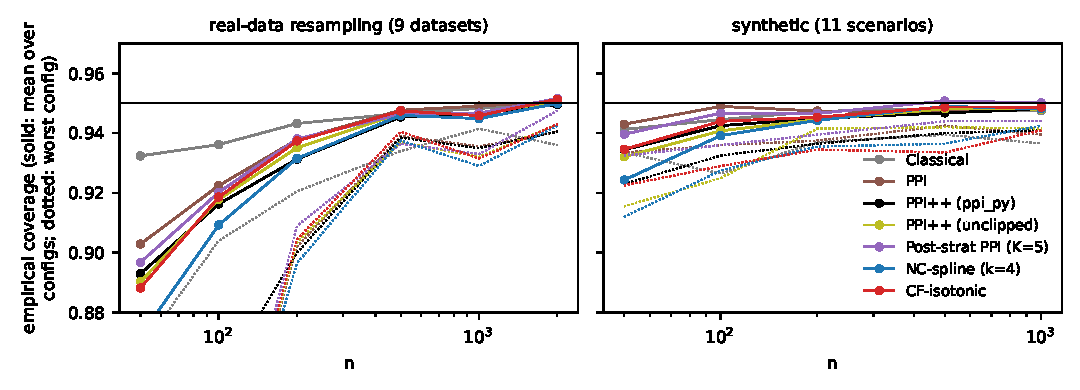
\includegraphics[width=0.95\linewidth]{figs/fig_coverage.pdf}
\caption{Empirical coverage vs $n$ averaged over settings (solid) and worst setting (dotted).}\label{fig:cover}
\end{figure}

\paragraph{Stress test: predictor scores on a different scale.}
The stored predictors are close to calibrated, which is why Table~\ref{tab:real} shows no headroom. To probe the opposite regime on real outcomes we keep each real pool and predictor but change the \emph{scale} on which its output is reported by a fixed monotone map (rank-uniformised score $T(f)=\mathrm{rank}(f)/(\text{pool}+1)$, or exponential scale $T(f)=\exp((f-\bar f)/s_f)$); this is a semi-synthetic stress test (7 datasets with continuous scores, $R=1000$, $N=10^4$). At $n=200$ (Table~\ref{tab:distort}) the NC-spline is 2--35\% shorter than unclipped PPI++ (median 6\%; largest: gene expression 0.65 on the exponential scale and AlphaFold 0.75 on the rank scale), tracking the bound (e.g.\ gene expression 0.315 vs.\ 0.317), and where the $\lambda$ clip also binds it is up to 54\% shorter than \texttt{ppi\_py} PPI++. Coverage of the NC-spline is 0.897--0.952 (mean 0.941 over 28 settings, lowest on heavy-tailed census income at $n=200$). Thus nonlinear controls matter when the predictor's output is not on an affine-calibrated scale, but the stored predictors happen not to be of that kind.

\begin{table}[t]
\centering\small
\caption{Score-scale stress test at $n=200$, $N=10^4$, $R=1000$: width relative to PPI++ (\texttt{ppi\_py}) of unclipped PPI++ and the NC-spline, the efficiency bound, and the NC-spline's coverage. $n=1000$ in \texttt{results/distort\_summary.csv}.}\label{tab:distort}
\resizebox{\linewidth}{!}{\begin{tabular}{lrrrrrrrr}
\toprule
 & \multicolumn{4}{c}{rank-uniformised score} & \multicolumn{4}{c}{exponential score scale} \\
Dataset & PPI++ unclip. & NC-spline & Bound & cov. NC-s. & PPI++ unclip. & NC-spline & Bound & cov. NC-s. \\
\midrule
Galaxies & 1.001 & 0.879 & 0.881 & 0.939 & 0.993 & 0.945 & 0.947 & 0.938 \\
Forest & 1.002 & 0.944 & 0.922 & 0.946 & 0.987 & 0.966 & 0.962 & 0.939 \\
AlphaFold & 1.002 & 0.749 & 0.720 & 0.921 & 0.980 & 0.916 & 0.937 & 0.952 \\
Gene expr. & 0.398 & 0.315 & 0.317 & 0.947 & 0.707 & 0.462 & 0.463 & 0.936 \\
Census income & 0.831 & 0.797 & 0.797 & 0.920 & 0.859 & 0.768 & 0.797 & 0.897 \\
Census health & 0.999 & 0.947 & 0.948 & 0.932 & 1.002 & 0.963 & 0.965 & 0.947 \\
Census educ. & 0.841 & 0.814 & 0.815 & 0.942 & 0.943 & 0.882 & 0.879 & 0.936 \\
\bottomrule
\end{tabular}}
\end{table}

\paragraph{Using covariates in addition to the prediction.}
For the three census collections we also tried a cross-fitted gradient-boosting control on $(f,X)$ with the covariates $X$ shipped with the data ($R=500$, Table~\ref{tab:extx}). The cross-fitted residual variance on the pool falls by only $0.6\%$, $0.1\%$ and $0.2\%$ (income, insurance, education) when $X$ is added to $f$, and the resulting intervals are $1.5$--$7.7\%$ \emph{wider} than PPI++ (coverage similar), so there is no gain from using $X$ in this way; the cost of fitting a flexible model on $n\le2000$ labels exceeds what it can learn.

\paragraph{Distribution shift (negative result).}
We drew labeled points from the 2013 plankton labels and unlabeled points from the 2014 predictions (truth = mean of the 2014 labels, $0.0714$), $N=10^4$, $R=2000$. The classical interval, which ignores the unlabeled data, fails as expected (coverage $0.262$ at $n=200$, $0.000$ at $n=1000$). PPI with $\lambda=1$ stays valid ($0.941$, $0.940$) because the predictor's error is similar in both years; but PPI++ with an unclipped tuned $\lambda<1$ (identical to the NC-spline on this binary predictor) is shorter and keeps $0.945$ at $n=200$ yet collapses to $0.578$ at $n=1000$ (bias $+0.011$ against a standard error of about $0.006$). The \texttt{ppi\_py} PPI++ has the same coverage and width as PPI here, i.e.\ its tuned $\lambda$ was clipped to 1. Tuning $\lambda$ below 1 trades the calibration-under-shift robustness of PPI for width, so the gain of shortening intervals is conditional on exchangeability, which none of the methods can verify from the data (no-shift control: $0.933$--$0.954$ for all methods, Table~\ref{tab:shift}).

\paragraph{Deployment example.} For ballots with the real split ($n=1027$ labels, $N=78{,}150$ unlabeled), the classical 95\% interval has width $0.0591$ while PPI, PPI++ and all our variants have width $0.0131$--$0.0133$ (estimate $0.6214$, $[0.6148,0.6280]$ for NC-spline); no variant of ours changes it (binary predictor). There is no ground truth for the unlabeled part, so this is illustrative only.

\section{Discussion and limitations}
\textbf{Answer to the question.} With labels, unlabeled data and predictor fixed, the headroom for the mean beyond a properly tuned (unclipped) PPI++ is $(1+\Gamma)^{-1/2}$ in width and is exactly zero when $\E[Y|f]$ is affine in $f$. On the nine real collections it is at most about 2\% (typically below 1\%), so we do not recommend nonlinear controls there; the benefit lies elsewhere (using $\lambda$ above 1 where needed; PPI itself). On predictors with miscalibrated or non-monotone scores, or scores on an arbitrary scale, the headroom is large (7--27\% in our synthetic scenarios) and reachable with a four-knot spline control at $n\gtrsim200$ without losing coverage.

\textbf{Limitations.} (1) Target: only the mean; quantiles, regression coefficients and other M-estimands are untested, and our theory is for the mean. (2) Real-data experiments resample with replacement from a finite pool and treat its mean as truth, so they test the estimators under i.i.d.\ sampling from the empirical distribution, not real sampling frames; the plankton and ballots pools are the stored labeled portions only. (3) Headroom for real data uses cross-fitted boosting for $\E v$ and is a plug-in estimate with no confidence interval. (4) Wald-type intervals are used throughout; small-$n$ undercoverage is documented but not solved (ballots, heavy-tailed income); bootstrap or exact methods were not tried. (5) The efficiency statement is argued, not proved, beyond within-class optimality. (6) $k=4$ and 5-fold cross-fitting were fixed in advance; sensitivity to $k\in\{3,6\}$ is in the released CSV but not tuned; the spline is clearly too small for heavy exponential $g$. (7) No multiplicity correction; the conclusions are about consistent patterns, not individual tests. (8) Our extension with covariates uses a boosting model fitted on the labeled data, which departs from a strictly ``fixed'' predictor. (9) Predictors are those shipped with the data; we did not study predictors of varying quality.

\textbf{Broader impact.} The work is methodological and uses public, de-identified data; the main risk is that shorter intervals presented without a coverage check (as at small $n$ here) overstate certainty.

\label{endmain}
\bibliographystyle{plainnat}
\bibliography{refs}

\appendix
\section{Proofs and derivations}\label{app:proofs}

Throughout, $(f_i,Y_i)_{i\le n}$ and $(f_j)_{j\le N}$ are i.i.d.\ from the same distribution, $g(f)=\E[Y\mid f]$, $v(f)=\Var(Y\mid f)$, and all second moments are finite. For $h$ with $\E h(f)^2<\infty$ let
$\hat\theta_h=\frac1n\sum_{i\le n}(Y_i-h(f_i))+\frac1N\sum_{j\le N}h(f_j)$.

\paragraph{Proof of Proposition~\ref{prop:main}.}
$\hat\theta_h$ is the sum of two independent sample means, hence unbiased for $\theta=\E Y$ with
$\Var(\hat\theta_h)=V(h):=\Var(Y-h)/n+\Var(h)/N$ exactly, and asymptotically normal as $n,N\to\infty$ by the Lindeberg--Feller CLT applied to each mean (with $n/N$ bounded).
Since $Y-g(f)$ is uncorrelated with every square-integrable function of $f$, $\Var(Y-h)=\E v+\Var(g-h)$. Write $h=cg+\delta$ with $c=N/(n+N)$ (so $1-c=n/(n+N)$). Then
$\Var(g-h)=(1-c)^2\Var g-2(1-c)\Cov(g,\delta)+\Var\delta$ and $\Var(h)=c^2\Var g+2c\Cov(g,\delta)+\Var\delta$, so
\[
V(h)=\frac{\E v}{n}+\Big[\frac{(1-c)^2}{n}+\frac{c^2}{N}\Big]\Var g+2\Big[\frac{c}{N}-\frac{1-c}{n}\Big]\Cov(g,\delta)+\Big(\frac1n+\frac1N\Big)\Var\delta .
\]
With $c=N/(n+N)$: $(1-c)^2/n+c^2/N=1/(n+N)$ and $c/N=(1-c)/n=1/(n+N)$, so the cross term vanishes and $V(h)=V_\star+(1/n+1/N)\Var(h-cg)$. \qed

\paragraph{Proof of Corollary~\ref{cor:lin}.}
For $h=\lambda f$, $\min_\lambda\Var(\lambda f-cg)=c^2\Var(g)(1-\rho^2)$ with $\rho=\mathrm{Corr}(g(f),f)$ (residual variance of the linear projection of $cg$ on $f$). By Proposition~\ref{prop:main}, $V_{\rm lin}-V_\star=(1/n+1/N)c^2\Var(g)(1-\rho^2)$, and $(1/n+1/N)c^2=\frac{n+N}{nN}\frac{N^2}{(n+N)^2}=\frac{N}{n(n+N)}$. Thus $V_{\rm lin}-V_\star=\frac{N}{n(n+N)}\Var(g)(1-\rho^2)$.
For the classical estimator ($h=0$), $V_0=\Var Y/n=(\E v+\Var g)/n$ and $V_0-V_\star=\Var(g)\big(\frac1n-\frac1{n+N}\big)=\frac{N}{n(n+N)}\Var g$; hence $(V_0-V_{\rm lin})/(V_0-V_\star)=\rho^2$. The width ratio statement follows from $\text{width}\propto\sqrt{V}$. For the expression of $\Gamma$: $V_{\rm lin}/V_\star=1+\Gamma$ with
$\Gamma=\frac{N\Var g\,(1-\rho^2)}{(n+N)\E v+n\Var g}$. \qed

\paragraph{Proof of Corollary~\ref{cor:clip}.}
$V(\lambda f)$ is quadratic in $\lambda$ with leading coefficient $(1/n+1/N)\Var f$ and minimiser $\lambda^\star=\Cov(g,f)/\big((1+n/N)\Var f\big)$, hence $V(\lambda f)=V(\lambda^\star f)+(1/n+1/N)\Var(f)(\lambda-\lambda^\star)^2$. Taking $\lambda=\mathrm{clip}(\lambda^\star,0,1)$ gives the stated excess when $\lambda^\star>1$ (or $<0$). \qed

\paragraph{Remark on efficiency (not a full proof).}
Let $R_k\in\{0,1\}$ indicate labeling, $\pi=n/(n+N)$ known and independent of $(f,Y)$. The observed-data model is then nonparametric for the law of $(f,Y)$, so there is a single influence function, $\varphi=\frac{R}{\pi}(Y-g(f))+g(f)-\theta$, whose variance divided by $n+N$ is $\frac{\E v}{\pi(n+N)}+\frac{\Var g}{n+N}=V_\star$. The estimator $\hat\theta_{cg}$ attains this value, which is why we call $V_\star$ the efficiency bound for this information structure (labels MCAR; $f$ observed everywhere). We use it as the benchmark for the headroom; the claims of the paper do not depend on its optimality beyond the elementary within-class optimality in Proposition~\ref{prop:main}.

\paragraph{Heuristic for the cost of estimating the controls.}
With $p$ estimated control coefficients, the classical regression-adjustment literature gives a relative variance inflation of order $p/n$ for the point estimator, and the in-sample residual variance is biased downwards by a factor of order $(n-p-1)/n$; the plug-in Wald interval is therefore too short by about the same relative amount. We do not derive this here; the data in Section~\ref{sec:exp} are used to check its qualitative implication (undercoverage of the richer control sets at small $n$, partly repaired by the degrees-of-freedom correction).


\section{Additional results and reproducibility}\label{app:extra}
\begin{figure}[h]
\centering
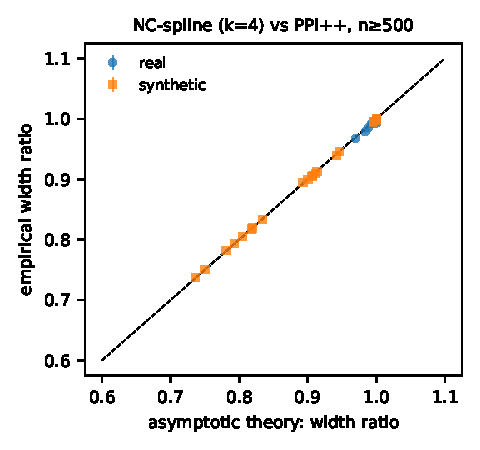
\includegraphics[width=0.45\linewidth]{figs/fig_theory_vs_emp.pdf}
\caption{Asymptotic prediction vs empirical width ratio of the NC-spline to PPI++ for $n\ge500$ (real and synthetic settings).}
\end{figure}
\begin{table}[h]
\centering\small
\caption{Plankton: distribution shift (labeled 2013, unlabeled and target 2014) and no-shift control; $N=10^4$, $R=2000$; the interval is the Wilson interval for the coverage.}\label{tab:shift}
\resizebox{\linewidth}{!}{\begin{tabular}{llrrrrr}
\toprule
Setting & $n$ & Method & Coverage & 95\% CI of cov. & Width & Bias \\
\midrule
shift(2013$\to$2014) & 200 & Classical & 0.262 & [0.243, 0.282] & 0.0940 & +0.0621 \\
shift(2013$\to$2014) & 200 & PPI & 0.941 & [0.930, 0.951] & 0.0541 & -0.0018 \\
shift(2013$\to$2014) & 200 & PPI++ (\texttt{ppi\_py}) & 0.941 & [0.929, 0.950] & 0.0540 & -0.0018 \\
shift(2013$\to$2014) & 200 & NC-spline (k=4) & 0.945 & [0.934, 0.954] & 0.0516 & +0.0089 \\
\midrule
shift(2013$\to$2014) & 1000 & Classical & 0.000 & [0.000, 0.002] & 0.0422 & +0.0625 \\
shift(2013$\to$2014) & 1000 & PPI & 0.940 & [0.928, 0.949] & 0.0258 & -0.0014 \\
shift(2013$\to$2014) & 1000 & PPI++ (\texttt{ppi\_py}) & 0.940 & [0.928, 0.949] & 0.0258 & -0.0014 \\
shift(2013$\to$2014) & 1000 & NC-spline (k=4) & 0.578 & [0.556, 0.599] & 0.0244 & +0.0112 \\
\midrule
no-shift control(2013) & 200 & Classical & 0.950 & [0.939, 0.958] & 0.0944 & +0.0012 \\
no-shift control(2013) & 200 & PPI & 0.949 & [0.938, 0.958] & 0.0548 & +0.0001 \\
no-shift control(2013) & 200 & PPI++ (\texttt{ppi\_py}) & 0.933 & [0.921, 0.943] & 0.0530 & -0.0023 \\
no-shift control(2013) & 200 & NC-spline (k=4) & 0.940 & [0.928, 0.949] & 0.0521 & +0.0002 \\
\midrule
no-shift control(2013) & 1000 & Classical & 0.943 & [0.932, 0.952] & 0.0421 & -0.0003 \\
no-shift control(2013) & 1000 & PPI & 0.954 & [0.943, 0.962] & 0.0274 & +0.0001 \\
no-shift control(2013) & 1000 & PPI++ (\texttt{ppi\_py}) & 0.950 & [0.939, 0.958] & 0.0255 & -0.0006 \\
no-shift control(2013) & 1000 & NC-spline (k=4) & 0.952 & [0.942, 0.961] & 0.0254 & -0.0001 \\
\bottomrule
\end{tabular}}
\end{table}
\begin{table}[h]
\centering\small
\caption{Pool statistics: $g=\E[Y|f]$ is exact for discrete $f$ and 10-fold cross-fitted boosting otherwise; $\rho^2=\mathrm{Corr}(g,f)^2$; $\lambda^\star$: unclipped optimal PPI++ coefficient at $n=200$, $N=10^4$ (values above 1 are clipped by \texttt{ppi\_py}).}\label{tab:pool}
\resizebox{\linewidth}{!}{\begin{tabular}{lrrrrrr}
\toprule
Dataset & pool & distinct $f$ & Corr$(Y,f)$ & $\mathrm{Var}(g)/\mathrm{Var}(Y)$ & $\rho^2$ & $\lambda^\star$ ($n{=}200$) \\
\midrule
Galaxies & 16,743 & $>10^2$ & 0.741 & 0.546 & 0.997 & 0.95 \\
Forest & 1,596 & $>10^2$ & 0.537 & 0.276 & 0.908 & 0.82 \\
AlphaFold & 10,802 & $>10^2$ & 0.815 & 0.663 & 0.990 & 1.01 \\
Gene expr. & 61,150 & $>10^2$ & 0.963 & 0.930 & 0.998 & 1.13 \\
Census income & 380,091 & $>10^2$ & 0.607 & 0.372 & 0.990 & 1.35 \\
Census health & 318,215 & $>10^2$ & 0.707 & 0.500 & 0.999 & 0.97 \\
Census educ. & 318,215 & $>10^2$ & 0.626 & 0.392 & 0.998 & 0.96 \\
Plankton & 421,238 & 2 & 0.836 & 0.699 & 1.000 & 0.83 \\
Ballots & 1,027 & 2 & 0.982 & 0.963 & 1.000 & 0.96 \\
\bottomrule
\end{tabular}}
\end{table}
\begin{table}[h]
\centering\small
\caption{Covariate extension ($N=10^4$, $R=500$): width ratio to PPI++ (\texttt{ppi\_py}) of the NC-spline, CF-isotonic and cross-fitted boosting on $(f,X)$ (paired mean $\pm$ SE), and coverage.}\label{tab:extx}
\resizebox{\linewidth}{!}{\begin{tabular}{lrrrrrr}
\toprule
Dataset & $n$ & NC-spline & CF-iso & CF-GBM$(f,X)$ & cov. PPI++ & cov. CF-GBM \\
\midrule
Census income & 200 & 0.967 & 1.028 & 1.067$\pm$0.002 & 0.910 & 0.910 \\
Census income & 1000 & 0.986 & 1.007 & 1.023$\pm$0.001 & 0.946 & 0.944 \\
Census income & 2000 & 0.994 & 1.006 & 1.016$\pm$0.000 & 0.954 & 0.954 \\
Census health & 200 & 0.994 & 1.027 & 1.069$\pm$0.002 & 0.970 & 0.972 \\
Census health & 1000 & 0.999 & 1.008 & 1.029$\pm$0.000 & 0.938 & 0.932 \\
Census health & 2000 & 0.999 & 1.004 & 1.015$\pm$0.000 & 0.948 & 0.942 \\
Census educ. & 200 & 0.993 & 1.033 & 1.077$\pm$0.002 & 0.936 & 0.930 \\
Census educ. & 1000 & 0.999 & 1.011 & 1.031$\pm$0.001 & 0.952 & 0.952 \\
Census educ. & 2000 & 1.000 & 1.006 & 1.017$\pm$0.000 & 0.962 & 0.954 \\
\bottomrule
\end{tabular}}
\end{table}
\begin{table}[h]
\centering\small
\caption{Ballots with the real split ($n=1027$, $N=78{,}150$): estimates and 95\% intervals (no ground truth for the unlabeled part).}\label{tab:ballots}
\begin{tabular}{lrrrr}
\toprule
Method & Estimate & Lower & Upper & Width \\
\midrule
Classical & 0.6280 & 0.5985 & 0.6576 & 0.0591 \\
PPI & 0.6211 & 0.6145 & 0.6278 & 0.0133 \\
PPI++ (\texttt{ppi\_py}) & 0.6214 & 0.6149 & 0.6280 & 0.0131 \\
PPI++ (unclipped) & 0.6214 & 0.6148 & 0.6280 & 0.0131 \\
Post-strat PPI (K=5) & 0.6213 & 0.6146 & 0.6280 & 0.0133 \\
NC-spline (k=4) & 0.6214 & 0.6148 & 0.6280 & 0.0131 \\
CF-isotonic & 0.6213 & 0.6147 & 0.6279 & 0.0132 \\
\bottomrule
\end{tabular}
\end{table}

\paragraph{Reproducibility.} Environment: Python 3.11.15, numpy 2.4.6, scipy 1.17.1, pandas 3.0.6, scikit-learn 1.9.1, matplotlib 3.11.2, ppi-python 0.2.3, joblib 1.6.0. All numbers, tables and figures are produced by scripts in \texttt{code/} (see \texttt{README.md}): \texttt{run\_real.py} (Table~\ref{tab:real}, Fig.~\ref{fig:real}), \texttt{run\_synth.py} (Table~\ref{tab:synth}, Fig.~\ref{fig:synth}), \texttt{run\_extra.py} (shift, ballots, covariates), \texttt{run\_distort.py} (score-scale stress test), \texttt{make\_figs.py} (all figures and tables). Seeds are derived from fixed base seeds. A first version of the post-stratified baseline ignored the randomness of the stratum shares and undercovered badly; it was fixed before the reported runs and all reported results come from the fixed code.

\paragraph{Disclosure of LLM use.} This study (design, implementation, experiments, analysis and drafting of the manuscript) was carried out by an autonomous LLM-based research agent working unattended; no human edited the results. No LLM is part of the statistical methods studied. The literature was limited to the starter list and the \texttt{ppi-python} source; arXiv metadata (titles, authors, dates) of the cited items was verified through the public arXiv API (\texttt{code/check\_refs.py}); no full texts were read.

\newpage
\section*{NeurIPS Paper Checklist}




\begin{enumerate}

\item {\bf Claims}
    \item[] Question: Do the main claims made in the abstract and introduction accurately reflect the paper's contributions and scope?
    \item[] Answer: \answerYes{} % Replace by \answerYes{}, \answerNo{}, or \answerNA{}.
    \item[] Justification: Abstract and introduction state the headroom analysis, the estimators, and the conditional empirical findings (Sections 3--5); the scope is the population mean only, stated in Sections 3 and 6.
    \item[] Guidelines:
    \begin{itemize}
        \item The answer \answerNA{} means that the abstract and introduction do not include the claims made in the paper.
        \item The abstract and/or introduction should clearly state the claims made, including the contributions made in the paper and important assumptions and limitations. A \answerNo{} or \answerNA{} answer to this question will not be perceived well by the reviewers. 
        \item The claims made should match theoretical and experimental results, and reflect how much the results can be expected to generalize to other settings. 
        \item It is fine to include aspirational goals as motivation as long as it is clear that these goals are not attained by the paper. 
    \end{itemize}

\item {\bf Limitations}
    \item[] Question: Does the paper discuss the limitations of the work performed by the authors?
    \item[] Answer: \answerYes{} % Replace by \answerYes{}, \answerNo{}, or \answerNA{}.
    \item[] Justification: Section 6 lists limitations (target limited to the mean, resampling protocol, plug-in headroom estimate, Wald intervals and small-$n$ undercoverage, efficiency statement argued rather than proved, no multiplicity correction).
    \item[] Guidelines:
    \begin{itemize}
        \item The answer \answerNA{} means that the paper has no limitation while the answer \answerNo{} means that the paper has limitations, but those are not discussed in the paper. 
        \item The authors are encouraged to create a separate ``Limitations'' section in their paper.
        \item The paper should point out any strong assumptions and how robust the results are to violations of these assumptions (e.g., independence assumptions, noiseless settings, model well-specification, asymptotic approximations only holding locally). The authors should reflect on how these assumptions might be violated in practice and what the implications would be.
        \item The authors should reflect on the scope of the claims made, e.g., if the approach was only tested on a few datasets or with a few runs. In general, empirical results often depend on implicit assumptions, which should be articulated.
        \item The authors should reflect on the factors that influence the performance of the approach. For example, a facial recognition algorithm may perform poorly when image resolution is low or images are taken in low lighting. Or a speech-to-text system might not be used reliably to provide closed captions for online lectures because it fails to handle technical jargon.
        \item The authors should discuss the computational efficiency of the proposed algorithms and how they scale with dataset size.
        \item If applicable, the authors should discuss possible limitations of their approach to address problems of privacy and fairness.
        \item While the authors might fear that complete honesty about limitations might be used by reviewers as grounds for rejection, a worse outcome might be that reviewers discover limitations that aren't acknowledged in the paper. The authors should use their best judgment and recognize that individual actions in favor of transparency play an important role in developing norms that preserve the integrity of the community. Reviewers will be specifically instructed to not penalize honesty concerning limitations.
    \end{itemize}

\item {\bf Theory assumptions and proofs}
    \item[] Question: For each theoretical result, does the paper provide the full set of assumptions and a complete (and correct) proof?
    \item[] Answer: \answerYes{} % Replace by \answerYes{}, \answerNo{}, or \answerNA{}.
    \item[] Justification: Proposition 1 and Corollaries 1--2 are proved in Appendix A with assumptions stated in Section 3 (i.i.d.\ sampling, finite second moments); the efficiency-bound statement is explicitly marked as argued, not proved.
    \item[] Guidelines:
    \begin{itemize}
        \item The answer \answerNA{} means that the paper does not include theoretical results. 
        \item All the theorems, formulas, and proofs in the paper should be numbered and cross-referenced.
        \item All assumptions should be clearly stated or referenced in the statement of any theorems.
        \item The proofs can either appear in the main paper or the supplemental material, but if they appear in the supplemental material, the authors are encouraged to provide a short proof sketch to provide intuition. 
        \item Inversely, any informal proof provided in the core of the paper should be complemented by formal proofs provided in appendix or supplemental material.
        \item Theorems and Lemmas that the proof relies upon should be properly referenced. 
    \end{itemize}

    \item {\bf Experimental result reproducibility}
    \item[] Question: Does the paper fully disclose all the information needed to reproduce the main experimental results of the paper to the extent that it affects the main claims and/or conclusions of the paper (regardless of whether the code and data are provided or not)?
    \item[] Answer: \answerYes{} % Replace by \answerYes{}, \answerNo{}, or \answerNA{}.
    \item[] Justification: Estimators (Section 4), protocol and metrics (Section 5), software versions and scripts (Appendix B and README) are fully specified.
    \item[] Guidelines:
    \begin{itemize}
        \item The answer \answerNA{} means that the paper does not include experiments.
        \item If the paper includes experiments, a \answerNo{} answer to this question will not be perceived well by the reviewers: Making the paper reproducible is important, regardless of whether the code and data are provided or not.
        \item If the contribution is a dataset and\slash or model, the authors should describe the steps taken to make their results reproducible or verifiable. 
        \item Depending on the contribution, reproducibility can be accomplished in various ways. For example, if the contribution is a novel architecture, describing the architecture fully might suffice, or if the contribution is a specific model and empirical evaluation, it may be necessary to either make it possible for others to replicate the model with the same dataset, or provide access to the model. In general. releasing code and data is often one good way to accomplish this, but reproducibility can also be provided via detailed instructions for how to replicate the results, access to a hosted model (e.g., in the case of a large language model), releasing of a model checkpoint, or other means that are appropriate to the research performed.
        \item While NeurIPS does not require releasing code, the conference does require all submissions to provide some reasonable avenue for reproducibility, which may depend on the nature of the contribution. For example
        \begin{enumerate}
            \item If the contribution is primarily a new algorithm, the paper should make it clear how to reproduce that algorithm.
            \item If the contribution is primarily a new model architecture, the paper should describe the architecture clearly and fully.
            \item If the contribution is a new model (e.g., a large language model), then there should either be a way to access this model for reproducing the results or a way to reproduce the model (e.g., with an open-source dataset or instructions for how to construct the dataset).
            \item We recognize that reproducibility may be tricky in some cases, in which case authors are welcome to describe the particular way they provide for reproducibility. In the case of closed-source models, it may be that access to the model is limited in some way (e.g., to registered users), but it should be possible for other researchers to have some path to reproducing or verifying the results.
        \end{enumerate}
    \end{itemize}


\item {\bf Open access to data and code}
    \item[] Question: Does the paper provide open access to the data and code, with sufficient instructions to faithfully reproduce the main experimental results, as described in supplemental material?
    \item[] Answer: \answerYes{} % Replace by \answerYes{}, \answerNo{}, or \answerNA{}.
    \item[] Justification: All code, the download script for the public \texttt{ppi-python} example data (v0.2.3) and exact commands are provided in the supplementary material (anonymous); the data are not redistributed.
    \item[] Guidelines:
    \begin{itemize}
        \item The answer \answerNA{} means that paper does not include experiments requiring code.
        \item Please see the NeurIPS code and data submission guidelines (\url{https://neurips.cc/public/guides/CodeSubmissionPolicy}) for more details.
        \item While we encourage the release of code and data, we understand that this might not be possible, so \answerNo{} is an acceptable answer. Papers cannot be rejected simply for not including code, unless this is central to the contribution (e.g., for a new open-source benchmark).
        \item The instructions should contain the exact command and environment needed to run to reproduce the results. See the NeurIPS code and data submission guidelines (\url{https://neurips.cc/public/guides/CodeSubmissionPolicy}) for more details.
        \item The authors should provide instructions on data access and preparation, including how to access the raw data, preprocessed data, intermediate data, and generated data, etc.
        \item The authors should provide scripts to reproduce all experimental results for the new proposed method and baselines. If only a subset of experiments are reproducible, they should state which ones are omitted from the script and why.
        \item At submission time, to preserve anonymity, the authors should release anonymized versions (if applicable).
        \item Providing as much information as possible in supplemental material (appended to the paper) is recommended, but including URLs to data and code is permitted.
    \end{itemize}


\item {\bf Experimental setting/details}
    \item[] Question: Does the paper specify all the training and test details (e.g., data splits, hyperparameters, how they were chosen, type of optimizer) necessary to understand the results?
    \item[] Answer: \answerYes{} % Replace by \answerYes{}, \answerNo{}, or \answerNA{}.
    \item[] Justification: Sample sizes, replications, seeds, knot counts, folds and the $t$-correction are specified in Sections 4--5; $k=4$ and 5 folds were fixed before seeing real-data results, no hyperparameter was tuned on test outcomes.
    \item[] Guidelines:
    \begin{itemize}
        \item The answer \answerNA{} means that the paper does not include experiments.
        \item The experimental setting should be presented in the core of the paper to a level of detail that is necessary to appreciate the results and make sense of them.
        \item The full details can be provided either with the code, in appendix, or as supplemental material.
    \end{itemize}

\item {\bf Experiment statistical significance}
    \item[] Question: Does the paper report error bars suitably and correctly defined or other appropriate information about the statistical significance of the experiments?
    \item[] Answer: \answerYes{} % Replace by \answerYes{}, \answerNo{}, or \answerNA{}.
    \item[] Justification: Coverage is reported with Wilson 95\% intervals and widths as paired ratios with standard errors over $R=2000$ (500--1000 in extensions) resamples; no multiplicity correction is applied (stated).
    \item[] Guidelines:
    \begin{itemize}
        \item The answer \answerNA{} means that the paper does not include experiments.
        \item The authors should answer \answerYes{} if the results are accompanied by error bars, confidence intervals, or statistical significance tests, at least for the experiments that support the main claims of the paper.
        \item The factors of variability that the error bars are capturing should be clearly stated (for example, train/test split, initialization, random drawing of some parameter, or overall run with given experimental conditions).
        \item The method for calculating the error bars should be explained (closed form formula, call to a library function, bootstrap, etc.)
        \item The assumptions made should be given (e.g., Normally distributed errors).
        \item It should be clear whether the error bar is the standard deviation or the standard error of the mean.
        \item It is OK to report 1-sigma error bars, but one should state it. The authors should preferably report a 2-sigma error bar than state that they have a 96\% CI, if the hypothesis of Normality of errors is not verified.
        \item For asymmetric distributions, the authors should be careful not to show in tables or figures symmetric error bars that would yield results that are out of range (e.g., negative error rates).
        \item If error bars are reported in tables or plots, the authors should explain in the text how they were calculated and reference the corresponding figures or tables in the text.
    \end{itemize}

\item {\bf Experiments compute resources}
    \item[] Question: For each experiment, does the paper provide sufficient information on the computer resources (type of compute workers, memory, time of execution) needed to reproduce the experiments?
    \item[] Answer: \answerYes{} % Replace by \answerYes{}, \answerNo{}, or \answerNA{}.
    \item[] Justification: CPU only; wall-clock times of every experiment script on a shared 40-core, 250\,GB machine are given in the README (about one hour in total); exploratory smoke tests with fewer replications were also run.
    \item[] Guidelines:
    \begin{itemize}
        \item The answer \answerNA{} means that the paper does not include experiments.
        \item The paper should indicate the type of compute workers CPU or GPU, internal cluster, or cloud provider, including relevant memory and storage.
        \item The paper should provide the amount of compute required for each of the individual experimental runs as well as estimate the total compute. 
        \item The paper should disclose whether the full research project required more compute than the experiments reported in the paper (e.g., preliminary or failed experiments that didn't make it into the paper). 
    \end{itemize}
    
\item {\bf Code of ethics}
    \item[] Question: Does the research conducted in the paper conform, in every respect, with the NeurIPS Code of Ethics \url{https://neurips.cc/public/EthicsGuidelines}?
    \item[] Answer: \answerYes{} % Replace by \answerYes{}, \answerNo{}, or \answerNA{}.
    \item[] Justification: Public, de-identified data and a purely methodological analysis; no deviations from the Code of Ethics that we are aware of.
    \item[] Guidelines:
    \begin{itemize}
        \item The answer \answerNA{} means that the authors have not reviewed the NeurIPS Code of Ethics.
        \item If the authors answer \answerNo, they should explain the special circumstances that require a deviation from the Code of Ethics.
        \item The authors should make sure to preserve anonymity (e.g., if there is a special consideration due to laws or regulations in their jurisdiction).
    \end{itemize}


\item {\bf Broader impacts}
    \item[] Question: Does the paper discuss both potential positive societal impacts and negative societal impacts of the work performed?
    \item[] Answer: \answerYes{} % Replace by \answerYes{}, \answerNo{}, or \answerNA{}.
    \item[] Justification: Section 6 notes the benefit (cheaper valid inference) and the main risk (shorter intervals presented without coverage checks overstate certainty); no direct negative application.
    \item[] Guidelines:
    \begin{itemize}
        \item The answer \answerNA{} means that there is no societal impact of the work performed.
        \item If the authors answer \answerNA{} or \answerNo, they should explain why their work has no societal impact or why the paper does not address societal impact.
        \item Examples of negative societal impacts include potential malicious or unintended uses (e.g., disinformation, generating fake profiles, surveillance), fairness considerations (e.g., deployment of technologies that could make decisions that unfairly impact specific groups), privacy considerations, and security considerations.
        \item The conference expects that many papers will be foundational research and not tied to particular applications, let alone deployments. However, if there is a direct path to any negative applications, the authors should point it out. For example, it is legitimate to point out that an improvement in the quality of generative models could be used to generate Deepfakes for disinformation. On the other hand, it is not needed to point out that a generic algorithm for optimizing neural networks could enable people to train models that generate Deepfakes faster.
        \item The authors should consider possible harms that could arise when the technology is being used as intended and functioning correctly, harms that could arise when the technology is being used as intended but gives incorrect results, and harms following from (intentional or unintentional) misuse of the technology.
        \item If there are negative societal impacts, the authors could also discuss possible mitigation strategies (e.g., gated release of models, providing defenses in addition to attacks, mechanisms for monitoring misuse, mechanisms to monitor how a system learns from feedback over time, improving the efficiency and accessibility of ML).
    \end{itemize}
    
\item {\bf Safeguards}
    \item[] Question: Does the paper describe safeguards that have been put in place for responsible release of data or models that have a high risk for misuse (e.g., pre-trained language models, image generators, or scraped datasets)?
    \item[] Answer: \answerNA{} % Replace by \answerYes{}, \answerNo{}, or \answerNA{}.
    \item[] Justification: No models or scraped datasets with misuse risk are released.
    \item[] Guidelines:
    \begin{itemize}
        \item The answer \answerNA{} means that the paper poses no such risks.
        \item Released models that have a high risk for misuse or dual-use should be released with necessary safeguards to allow for controlled use of the model, for example by requiring that users adhere to usage guidelines or restrictions to access the model or implementing safety filters. 
        \item Datasets that have been scraped from the Internet could pose safety risks. The authors should describe how they avoided releasing unsafe images.
        \item We recognize that providing effective safeguards is challenging, and many papers do not require this, but we encourage authors to take this into account and make a best faith effort.
    \end{itemize}

\item {\bf Licenses for existing assets}
    \item[] Question: Are the creators or original owners of assets (e.g., code, data, models), used in the paper, properly credited and are the license and terms of use explicitly mentioned and properly respected?
    \item[] Answer: \answerYes{} % Replace by \answerYes{}, \answerNo{}, or \answerNA{}.
    \item[] Justification: Assets are credited and versions given (\texttt{ppi-python} 0.2.3, MIT licence for the code; the example \texttt{.npz} data files carry no separate licence statement in the package or PyPI page, so we use them only for research and do not redistribute them).
    \item[] Guidelines:
    \begin{itemize}
        \item The answer \answerNA{} means that the paper does not use existing assets.
        \item The authors should cite the original paper that produced the code package or dataset.
        \item The authors should state which version of the asset is used and, if possible, include a URL.
        \item The name of the license (e.g., CC-BY 4.0) should be included for each asset.
        \item For scraped data from a particular source (e.g., website), the copyright and terms of service of that source should be provided.
        \item If assets are released, the license, copyright information, and terms of use in the package should be provided. For popular datasets, \url{paperswithcode.com/datasets} has curated licenses for some datasets. Their licensing guide can help determine the license of a dataset.
        \item For existing datasets that are re-packaged, both the original license and the license of the derived asset (if it has changed) should be provided.
        \item If this information is not available online, the authors are encouraged to reach out to the asset's creators.
    \end{itemize}

\item {\bf New assets}
    \item[] Question: Are new assets introduced in the paper well documented and is the documentation provided alongside the assets?
    \item[] Answer: \answerYes{} % Replace by \answerYes{}, \answerNo{}, or \answerNA{}.
    \item[] Justification: The released code is documented in the README (environment, commands, runtimes, mapping from each table and figure to its script).
    \item[] Guidelines:
    \begin{itemize}
        \item The answer \answerNA{} means that the paper does not release new assets.
        \item Researchers should communicate the details of the dataset\slash code\slash model as part of their submissions via structured templates. This includes details about training, license, limitations, etc. 
        \item The paper should discuss whether and how consent was obtained from people whose asset is used.
        \item At submission time, remember to anonymize your assets (if applicable). You can either create an anonymized URL or include an anonymized zip file.
    \end{itemize}

\item {\bf Crowdsourcing and research with human subjects}
    \item[] Question: For crowdsourcing experiments and research with human subjects, does the paper include the full text of instructions given to participants and screenshots, if applicable, as well as details about compensation (if any)? 
    \item[] Answer: \answerNA{} % Replace by \answerYes{}, \answerNo{}, or \answerNA{}.
    \item[] Justification: No crowdsourcing or human-subjects research was conducted by us; the datasets are pre-existing public collections.
    \item[] Guidelines:
    \begin{itemize}
        \item The answer \answerNA{} means that the paper does not involve crowdsourcing nor research with human subjects.
        \item Including this information in the supplemental material is fine, but if the main contribution of the paper involves human subjects, then as much detail as possible should be included in the main paper. 
        \item According to the NeurIPS Code of Ethics, workers involved in data collection, curation, or other labor should be paid at least the minimum wage in the country of the data collector. 
    \end{itemize}

\item {\bf Institutional review board (IRB) approvals or equivalent for research with human subjects}
    \item[] Question: Does the paper describe potential risks incurred by study participants, whether such risks were disclosed to the subjects, and whether Institutional Review Board (IRB) approvals (or an equivalent approval/review based on the requirements of your country or institution) were obtained?
    \item[] Answer: \answerNA{} % Replace by \answerYes{}, \answerNo{}, or \answerNA{}.
    \item[] Justification: No human-subjects research was conducted by us.
    \item[] Guidelines:
    \begin{itemize}
        \item The answer \answerNA{} means that the paper does not involve crowdsourcing nor research with human subjects.
        \item Depending on the country in which research is conducted, IRB approval (or equivalent) may be required for any human subjects research. If you obtained IRB approval, you should clearly state this in the paper. 
        \item We recognize that the procedures for this may vary significantly between institutions and locations, and we expect authors to adhere to the NeurIPS Code of Ethics and the guidelines for their institution. 
        \item For initial submissions, do not include any information that would break anonymity (if applicable), such as the institution conducting the review.
    \end{itemize}

\item {\bf Declaration of LLM usage}
    \item[] Question: Does the paper describe the usage of LLMs if it is an important, original, or non-standard component of the core methods in this research? Note that if the LLM is used only for writing, editing, or formatting purposes and does \emph{not} impact the core methodology, scientific rigor, or originality of the research, declaration is not required.
    %this research? 
    \item[] Answer: \answerYes{} % Replace by \answerYes{}, \answerNo{}, or \answerNA{}.
    \item[] Justification: The research itself (design, code, experiments, analysis and drafting) was carried out by an autonomous LLM-based research agent; no LLM is part of the studied statistical methods. This is disclosed in Appendix B.
    \item[] Guidelines:
    \begin{itemize}
        \item The answer \answerNA{} means that the core method development in this research does not involve LLMs as any important, original, or non-standard components.
        \item Please refer to our LLM policy in the NeurIPS handbook for what should or should not be described.
    \end{itemize}

\end{enumerate}
\end{document}
